\documentclass[11pt]{article}

% --- Packages ---
\usepackage[french]{babel}
\usepackage[utf8]{inputenc}
\usepackage[T1]{fontenc}
\usepackage{amsmath,amssymb}
\usepackage{tikz}
\usepackage{graphicx}
\usepackage{booktabs}
\usepackage[margin=2.5cm]{geometry}
\usepackage{hyperref}
\usepackage{float}
\usepackage{textcomp}
\usepackage{textcomp}
\usepackage{caption}
\usepackage{cite}
\usetikzlibrary{positioning,arrows.meta,calc,shadows}

\linespread{1.08}

\begin{document}

% ---------------- Compact centered header with image between "Université de Kinshasa" and "Faculté ..." ----------------
\thispagestyle{empty}
\begin{center}
  {\bfseries\small RÉPUBLIQUE DÉMOCRATIQUE DU CONGO} \\[2pt]
  {\bfseries\small UNIVERSITÉ DE KINSHASA} \\[6pt]
  
\includegraphics[width=0.14\textwidth]{images.png} \\[6pt]
  {\small FACULTÉ DES SCIENCES ET TECHNOLOGIES \\ Mention Mathématiques, Statistique et Informatique} \\[2pt]
  {\small B.P. 190 KINSHASA XI} \\[6pt]
  {\small Master 1} \\[6pt]
  {\bfseries\large TRAVAIL PRATIQUE DE SYSTÈME MULTI-AGENT} \\[6pt]
  {\Large\bfseries Modélisation et Simulation d'une Épidémie \\[6pt]
  {\normalsize DUASENGE MAYANO BRUMMEL \\  3 Décembre 2025}}
\end{center}
\vspace{6pt} % très petit espace après l'en-tête

% --------------------------------- Corps du document ---------------------------------

\begin{abstract}
Ce travail propose la modélisation et la simulation d'une épidémie par contact dans une population. Le modèle compartimental SEIR étendu distingue cinq catégories : susceptibles (S), exposés (E), infectieux (I), guéris avec traitement (R$_1$) et spontanément (R$_2$). Le modèle intègre les rechutes et la perte d'immunité. Le système d'équations différentielles ordinaires est résolu numériquement par la méthode de Runge-Kutta d'ordre 4 implémentée dans GAMA Platform. Les simulations révèlent la dynamique temporelle des compartiments avec identification des pics épidémiques et de la distribution finale de la population.
\end{abstract}

\section{Introduction}

Les maladies contagieuses se propageant par contact direct ou indirect constituent des enjeux majeurs de santé publique en raison de leur capacité à générer des épidémies au sein des populations. La compréhension et la prédiction des dynamiques épidémiques sont essentielles pour mettre en place des stratégies de contrôle et de prévention efficaces. Les modèles mathématiques, et en particulier les modèles compartimentaux, se sont avérés indispensables pour analyser la propagation des maladies contagieuses et évaluer l'impact de différentes interventions. Ces approches remontent aux travaux fondateurs de Kermack et McKendrick~\cite{kermack1927}, qui ont posés les bases mathématique de la modélisation épidémiologique.

Ce travail considère une maladie contagieuse se propageant par contact dans une population quelconque. Le modèle compartimentalété proposé distingue cinq catégories de population selon leur statut épidémiologique : les \textbf{S\_people} représentent les personnes saines et susceptibles d'attraper la maladie suivant un taux de transmission $\lambda$ et devenir E\_people ; les \textbf{E\_people} sont les personnes exposées, ayant l'infection mais incapables de la transmettre, qui deviennent I\_people après un temps moyen déterminé par un taux de progression $\pi$ ; les \textbf{I\_people} sont les personnes infectieuses capables de transmettre la maladie ; les \textbf{R\_people1} représentent les personnes guéries après traitement suivant un taux de guérison $\gamma$ ; les \textbf{R\_people2} représentent les personnes guéries spontanément suivant un taux de guérison $\gamma_1$. De plus, le modèle intègre des mécanismes de rechute : les personnes R\_people1 et R\_people2 peuvent rechuter et redevenir E\_people si elles entrent en contact avec un I\_people, suivant respectivement des taux de rechute $\mathrm{rech}_1$ et $\mathrm{rech}_2$. Le modèle inclut également la perte progressive d'immunité : les personnes R\_people1 et R\_people2 peuvent redevenir S\_people après un temps donné suivant un taux de perte d'immunité $k$. Enfin, les populations intègrent des mécanismes démographiques : chaque compartiment subit une mortalité naturelle au taux $\mu_1$, tandis que les I\_people subissent également une mortalité liée à l'infection au taux $\mu_2$ ; un taux constant de recrutement $\Lambda$ alimente le compartiment S\_people avec de nouveaux individus susceptibles. Cette extension du modèle SEIR classique~\cite{hethcote2000} permet de capturer des dynamiques épidémiologiques complexes incluant les rechutes progressives et la perte graduelle d'immunité.

Face à cette problématique, ce travail poursuit trois objectifs principaux : (1)~établir le modèle compartimental représentant ces dynamiques épidémiologiques ; (2)~proposer une modélisation mathématique de ce modèle compartimental en utilisant les équations différentielles ordinaires (EDO) ; (3)~proposer un code GAML sous GAMA Platform simulant ces équations en les résolvant avec la méthode de Runge-Kutta d'ordre 4.

Le rapport est organisé comme suit. La section 2 présente le modèle compartimental et le diagramme de flux des transitions entre compartiments. La section 3 formalise le système d'équations différentielles ordinaires correspondant aux dynamiques du modèle. La section 4 détaille les paramètres et valeurs initiales utilisés pour les simulations. La section 5 décrit l'implémentation numérique en GAML et la résolution des EDO par la méthode de Runge-Kutta d'ordre 4. La section 6 présente les résultats des simulations et une analyse des dynamiques épidémiologiques observées. Finalement, la conclusion synthétise les principaux résultats et perspectives. La section suivante présente le modèle compartimental développé pour représenter ces interactions épidémiologiques complexes.

\section{Modèle Compartimental}\label{sec:modele_compartimental}

L'approche compartimentale divise la population en catégories homogènes selon leur statut épidémiologique. Le modèle SEIR étendu proposé distingue cinq compartiments, avec deux voies de récupération distinctes (R$_1$ pour guérison traitée et R$_2$ pour guérison spontanée) afin de capturer les rechutes et la perte progressive d'immunité. Cette extension du modèle SEIR classique~\cite{hethcote2000} permet de capturer des dynamiques épidémiologiques plus réalistes.

\subsection{Description des compartiments}

\textbf{S (Susceptibles)} : Individus sains alimentés par recrutement ($\Lambda$) et perte d'immunité ($k R_1 + k R_2$), diminuant par infection ($\lambda S I$) et mortalité naturelle ($\mu_1 S$).

\textbf{E (Exposés)} : Individus porteurs non-infectieux, alimentés par infection ($\lambda S I$) et rechutes ($\mathrm{rech}_1 R_1 I + \mathrm{rech}_2 R_2 I$), progressant vers infectiosité ($\pi E$).

\textbf{I (Infectieux)} : Individus transmetteurs, progressant des exposés ($\pi E$), sortant par guérison traitée ($\gamma I$), guérison spontanée ($\gamma_1 I$), ou mortalité ($\mu_1 I + \mu_2 I$).

\textbf{R$_1$ (Récupérés traités)} : Individus guéris par traitement, pouvant rechuter ($\mathrm{rech}_1 R_1 I$) ou perdre l'immunité ($k R_1$), subissant mortalité naturelle ($\mu_1 R_1$).

\textbf{R$_2$ (Récupérés spontanés)} : Individus guéris spontanément, avec dynamique similaire à R$_1$ : rechute ($\mathrm{rech}_2 R_2 I$), perte d'immunité ($k R_2$), mortalité naturelle ($\mu_1 R_2$).





\begin{figure}[H]
\centering
\resizebox{\textwidth}{!}{%
\begin{tikzpicture}[
  >=Stealth,
  comp/.style={
    draw=black, thick, rounded corners, minimum width=3.0cm, minimum height=1.1cm,
    align=center, font=\large\bfseries, text=white,
    drop shadow={shadow xshift=0.6mm, shadow yshift=-0.6mm}
  },
  arr/.style={->, thick, shorten >=2pt, shorten <=2pt},
  arrthin/.style={->, thin, shorten >=2pt, shorten <=2pt},
  labsmall/.style={font=\small}
]

% --- Compartiments alignés horizontalement
\node[comp, fill=green!60!black]  (S)  at (0,0)     {S\_people};
\node[comp, fill=orange!70!black] (E)  at (4,0)     {E\_people};
\node[comp, fill=red!80!black]    (I)  at (8,0)     {I\_people};
\node[comp, fill=blue!70!black]   (R1) at (12,0)    {R\_people1};
\node[comp, fill=purple!70!black] (R2) at (16,0)    {R\_people2};

% --- Recrutement Λ (CORRIGÉ: Λ au lieu de ΛN)
\coordinate (leftin) at (-2.2,0.25);
\draw[arr] (leftin) -- node[above,labsmall] {$\Lambda$} ($(S.west)+(0,0.25)$);

% --- Transitions principales (S->E, E->I, I->R1)
\draw[arr] (S.east) -- node[above,labsmall] {$\lambda S(t)I(t)$} ($(E.west)+(0,-0.03)$);
\draw[arr] (E.east) -- node[above,labsmall] {$\pi E(t)$} (I.west);
\draw[arr] (I.east) -- node[above,labsmall] {$\gamma I(t)$} (R1.west);

% --- gamma1 (I -> R2)
\draw[arr]
  ($(I.south east)+(0.05,-0.02)$) -- ++(0,-1.05) coordinate (g1_down)
                                 -- ++(3.0,0) node[midway,below=3pt,labsmall] {$\gamma_1 I(t)$}
                                 -- ($(R2.west)+(0,0.03)$);

% --- Mortalité μ1 ET μ2 from I (CORRIGÉ: ajout μ2 I)
\draw[arr]
  ($(I.south)+(-0.7,-0.03)$) -- ++(0,-1.05) node[below,labsmall] {$\mu_1 I$};
\draw[arrthin, red]
  ($(I.south)+(0.0,-0.03)$) -- ++(0,-1.05) node[below,labsmall] {$\mu_2 I$};

% --- Rechute R1 -> E
\draw[arr]
  (R1.north) -- ++(0,2.4) coordinate (R1_up)
            -- ($(E.north)+(-1.0,2.4)$) coordinate (E1_up)
            -- (E.north west);
\node[above,labsmall] at ($(R1_up)!0.5!(E1_up)$) {$\mathrm{rech}_1 R_1 I$};

% --- Rechute R2 -> E
\draw[arr]
  (R2.north) -- ++(0,3.6) coordinate (R2_up)
            -- ($(E.north)+(1.0,3.6)$) coordinate (E2_up)
            -- (E.north east);
\node[above,labsmall] at ($(R2_up)!0.5!(E2_up)$) {$\mathrm{rech}_2 R_2 I$};

% --- k R1 -> S (ligne pointillée)
\draw[->, dashed, thick]
  ($(R1.south)+(-0.35,0)$) -- ++(0,-1.8) coordinate (R1_down)
             -- ($(S.south)+(-1.0,-1.8)$) coordinate (S1_down)
             -- (S.south west);
\node[below,labsmall] at ($(R1_down)!0.5!(S1_down)$) {$k R_1$};

% --- μ1 R1
\draw[arr]
  ($(R1.south)+(0.45,-0.03)$) -- ++(0,-1.05) node[below,labsmall] {$\mu_1 R_1$};

% --- k R2 -> S (ligne pointillée)
\draw[->, dashed, thick]
  ($(R2.south)+(-0.35,0)$) -- ++(0,-2.6) coordinate (R2_down)
             -- ($(S.south)+(1.0,-2.6)$) coordinate (S2_down)
             -- (S.south east);
\node[below,labsmall] at ($(R2_down)!0.5!(S2_down)$) {$k R_2$};

% --- μ1 R2
\draw[arr]
  ($(R2.south)+(0.45,-0.03)$) -- ++(0,-1.05) node[below,labsmall] {$\mu_1 R_2$};

% --- mortalité naturelle μ1 sur S et E
\draw[arr] ($(S.south)+(0,-0.03)$) -- ++(0,-1.0) node[below,labsmall] {$\mu_1 S$};
\draw[arr] ($(E.south)+(0,-0.03)$) -- ++(0,-1.0) node[below,labsmall] {$\mu_1 E$};

\end{tikzpicture}
} % end resizebox
\caption{Diagramme compartimental SEIR1R2}
\label{fig:diagramme}
\end{figure}

Le diagramme de la Figure~\ref{fig:diagramme} synthétise l'ensemble des flux de transition entre les cinq compartiments. La section suivante traduit ces interactions en un système d'équations différentielles ordinaires permettant la simulation numérique.

\section{Formulation Mathématique}\label{sec:formulation}

Le modèle compartimental se traduit mathématiquement par un système d'équations différentielles ordinaires couplées. Chaque compartiment évolue selon les flux de transition définis à la Figure~\ref{fig:diagramme}. Le système d'équations suivant synthétise ces dynamiques :

\[
\left\{ \begin{aligned}
\frac{dS}{dt} &= \Lambda + k(R_1 + R_2) - \mu_1 S - \lambda S I, \\
\frac{dE}{dt} &= \lambda S I + \mathrm{rech}_1 R_1 I + \mathrm{rech}_2 R_2 I - (\pi + \mu_1) E, \\
\frac{dI}{dt} &= \pi E - (\gamma + \gamma_1 + \mu_1 + \mu_2) I, \\
\frac{dR_1}{dt} &= \gamma I - (\mathrm{rech}_1 I + k + \mu_1) R_1, \\
\frac{dR_2}{dt} &= \gamma_1 I - (\mathrm{rech}_2 I + k + \mu_1) R_2.
\end{aligned} \right.
\]

Ce système est résolu numériquement par la méthode de Runge-Kutta d'ordre 4. La résolution numérique nécessite la spécification des paramètres épidémiologiques présentés dans la section suivante.

\section{Paramètres du Modèle}\label{sec:parametres}

Le système d'équations différentielles ordinaires présenté à la section~\ref{sec:formulation} dépend entièrement de paramètres épidémiologiques spécifiques au pathogène et à la population considérée. La calibration précise de ces paramètres est essentielle pour obtenir des simulations réalistes reflétant les dynamiques observées sur le terrain.
Les paramètres épidémiologiques utilisés dans le modèle sont présentés dans le tableau suivant.


\begin{table}[h]
\centering
\caption{Paramètres épidémiologiques du modèle SEIR étendu.}
\label{tab:parametres}
\begin{tabular}{@{}lll@{}}
\toprule
Paramètre (symbole) & Description & Valeur (unité) \\
\midrule
$\Lambda$ & Taux de recrutement (natalité) & 0.00018 (jour$^{-1}$) \\
$\lambda$ & Taux de transmission & 0.0115 (jour$^{-1} \cdot$ pop$^{-1}$) \\
$\pi$ & Taux de progression E$\to$I & 0.09 (jour$^{-1}$) \\
$\gamma$ & Taux de guérison traitée I$\to$R1 & 0.05 (jour$^{-1}$) \\
$\gamma_1$ & Taux de guérison spontanée I$\to$R2 & 0.0714 (jour$^{-1}$) \\
$\mathrm{rech}_1$ & Taux de rechute R1$\to$E & 0.001 (jour$^{-1} \cdot$ pop$^{-1}$) \\
$\mathrm{rech}_2$ & Taux de rechute R2$\to$E & 0.002 (jour$^{-1} \cdot$ pop$^{-1}$) \\
$k$ & Taux de perte d'immunité $R_1, R_2 \to S$ & 0.01 (jour$^{-1}$) \\
$\mu_1$ & Taux de mortalité naturelle & $4.563 \times 10^{-5}$ (jour$^{-1}$) \\
$\mu_2$ & Taux de mortalité par infection & 0.0018 (jour$^{-1}$) \\
\bottomrule
\end{tabular}
\end{table}

L'implémentation numérique utilisant ces paramètres est détaillée dans la section suivanteon est détaillée ci-après.


\section{Implémentation Numérique et Simulation}\label{sec:implementation}

Le système d'équations différentielles ordinaires présenté à la section~\ref{sec:formulation} est résolu numériquement en utilisant la méthode de Runge-Kutta d'ordre 4 (RK4)~\cite{butcher2016}, reconnue pour son excellent compromis entre précision et efficacité computationnelle dans la résolution de systèmes d'EDO non-linéaires. L'implémentation est réalisée sur la plateforme GAMA (GIS and Agent-based Modelling Architecture)~\cite{taillandier2019, kasereka2025gama, kasereka2025sma}, un environnement de simulation multi-agent disposant de solveurs numériques intégrés pour la résolution d'EDO.

\subsection{Conditions initiales et paramètres de simulation}

Les conditions initiales modélisent l'introduction d'un cas index dans une population naïve : $S(0) = 100$ individus susceptibles, $I(0) = 1$ individu infectieux entrainant des contacts initiaux, et $E(0) = R_1(0) = R_2(0) = 0$. Ces conditions reflètent un scénario réaliste d'émergence épidémique au sein d'une petite population. La simulation est exécutée sur une durée de 132 jours, les paramètres épidémiologiques spécifiés à la section~\ref{sec:parametres} sont fixés pendant toute la durée de la simulation, sans intervention externe de contrôle.

\subsection{Architecture de la simulation GAMA}

La plateforme GAMA a été configurée avec une unique espèce agent \texttt{mathTB} encapsulant le système d'équations différentielles. L'agent gère les cinq états épidémiologiques $(S, E, I, R_1, R_2)$ mises à jour à chaque pas de temps par le solveur RK4 intégré. Les sorties graphiques générées incluent trois visualisations complémentaires : (i) une courbe temporelle montrant l'évolution conjointe des compartiments, (ii) un diagramme circulaire synthétisant la répartition finale, et (iii) un histogramme comparant les effectifs finaux. Le détail complet du code GAMA est présenté à l'Annexe~A (annexe~\ref{annexe:code_gama}).

Les résultats obtenus par cette implémentation numérique sont présentés et analysés dans la section suivante.


\section{Résultats de Simulation et Interprétation Graphique}\label{sec:resultats}

Cette section présente les résultats de simulation obtenus par résolution numérique du système SEIR étendu sur 132 jours. Trois aspects principaux sont analysés : l'évolution temporelle des compartiments, les pics épidémiques, et la distribution finale de la population.

\subsection{Évolution temporelle des compartiments}\label{subsec:dynamique_temporelle}

La Figure~\ref{fig:evolution} synthétise la dynamique temporelle des cinq compartiments sur 132 jours. Partant d'un seul infecté initial, la simulation a montré une propagation rapide suivant la séquence $S\to E\to I\to R$. La croissance initiale (jours 0--33) a été rapide : le compartiment exposé a atteint $\approx 47$ individus vers le jour 23, suivi du pic infectieux ($\approx 28$ individus) vers le jour 31, reflétant le délai d'incubation. Après le jour 50, une décroissance progressive a débuté, avec accumulation des individus guéris dans R$_1$ et R$_2$. Au-delà du jour 100, une circulation résiduelle a persisté due aux mécanismes de rechute et perte d'immunité.

\begin{figure}[H]
\centering
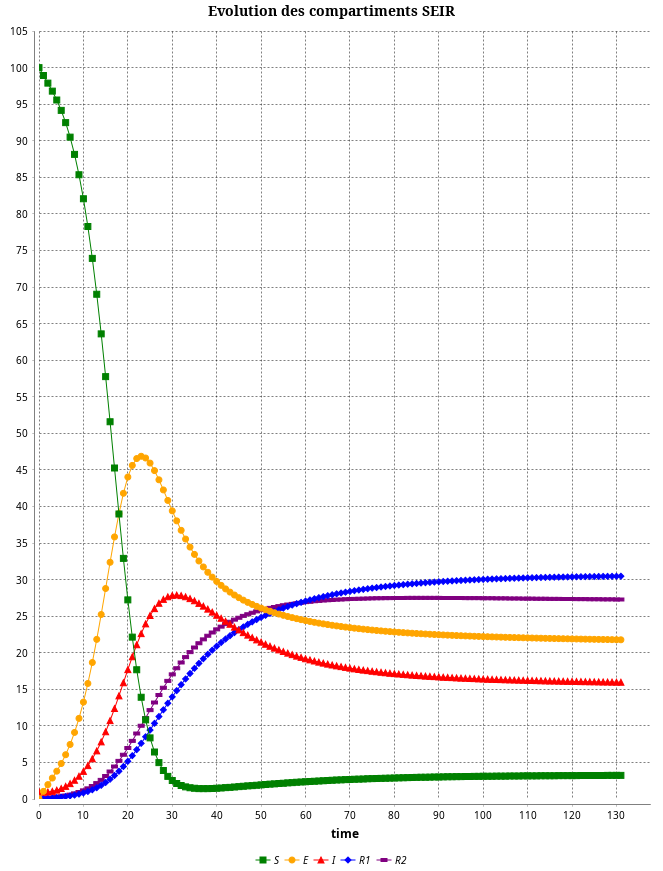
\includegraphics[width=0.85\textwidth]{epidemie_etendue_resultat_evolution.png}
\caption{Évolution temporelle des cinq compartiments du modèle SEIR étendu sur 132 jours. Les courbes représentent les susceptibles (S, vert), exposés (E, orange), infectieux (I, rouge), récupérés traités (R$_1$, bleu) et récupérés spontanés (R$_2$, violet).}
\label{fig:evolution}
\end{figure}

L'analyse quantitative des pics épidémiques observés permet d'identifier les paramètres clés contrôlant la dynamique.

\subsection{Analyse des pics épidémiques}\label{subsec:analyse_pics}

La Figure~\ref{fig:evolution} a montré un pic d'exposés ($\approx 47$ individus) vers le jour 23, suivi d'un pic infectieux ($\approx 28$ individus) vers le jour 31. Ce décalage de $\approx 8$ jours a reflété la période d'incubation ($1/\pi \approx 11$ jours) et la dynamique de progression $E \to I$. Les paramètres clés déterminant ces pics sont : (1) le taux de transmission $\lambda$, qui contrôle l'amplitude de la croissance initiale, (2) les taux de guérison $\gamma$ et $\gamma_1$, qui influencent la durée du pic infectieux, et (3) les taux de rechute et perte d'immunité, qui maintiennent une circulation résiduelle après le pic principal.

\subsection{Distribution finale des compartiments}\label{subsec:distribution_finale}

Au-delà de la dynamique transitoire, la distribution finale des compartiments a révélé l'impact cumulé de l'épidémie.

Au jour 132, la distribution des individus entre les cinq compartiments a reflété l'impact cumulé de la dynamique épidémique. Les Figures~\ref{fig:repartition} et~\ref{fig:histogramme} ont synthétisé cette répartition finale. À l'instant final, les valeurs étaient approximativement : $S \approx 4$ individus, $E \approx 22$, $I \approx 16$, $R_1 \approx 31$ et $R_2 \approx 28$. La majorité de la population se trouvait dans les compartiments des récupérés ($R_1 + R_2 \approx 59$ individus), tandis qu'une circulation résiduelle significative persistait ($E + I \approx 38$ individus). En tenant compte de la population totale à $t=132$, soit la population initiale de 101 individus plus le recrutement cumulé $\Lambda \cdot 132 = 0.00018 \times 132 \approx 0.024$, le taux d'attaque final était $(E + I + R_1 + R_2) / 101.024 = 97/101.024 \approx 96\%$, révélant qu'une fraction infime de susceptibles (seulement $S \approx 4$ sur 101 individus) persistait à la fin de la simulation.

\begin{figure}[H]
\centering
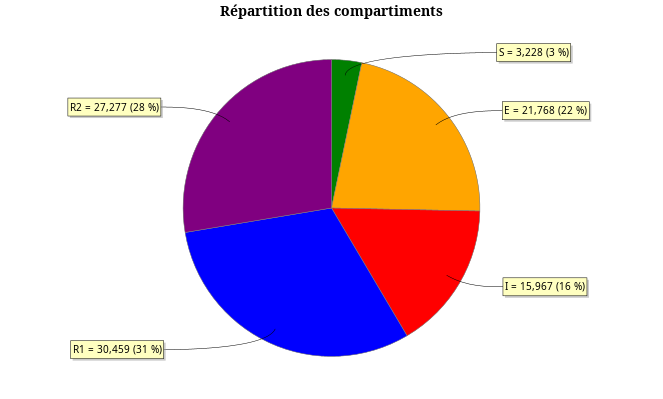
\includegraphics[width=0.85\textwidth]{epidemie_etendue_resultat_repartition.png}
\caption{Répartition proportionnelle des compartiments à t=132 jours.}
\label{fig:repartition}
\end{figure}

\begin{figure}[H]
\centering
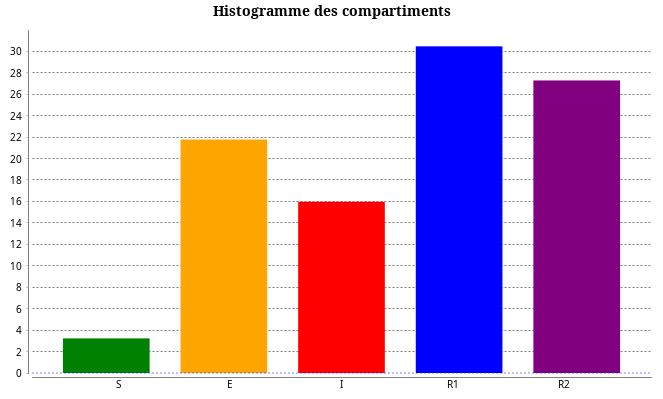
\includegraphics[width=0.85\textwidth]{epidemie_etendue_resultat_histogramme.png}
\caption{Effectifs finaux par compartiment à t=132 jours.}
\label{fig:histogramme}
\end{figure}


Le taux d'attaque très élevé (96\%) a reflété la transmissibilité importante du pathogène en l'absence de mesures de contrôle. Le ratio $R_2/R_1 \approx 0.9$ était cohérent avec les taux de guérison relatifs $\gamma_1/\gamma \approx 1.43$. La circulation résiduelle ($E+I \approx 38$ individus) a résulté des mécanismes de rechute et perte progressive d'immunité, indiquant une endémicité chronique à bas niveau plutôt qu'une extinction du pathogène.

\section{Conclusion}\label{sec:conclusion}
Ce travail a atteint les trois objectifs fixés notamment l'établissement d'un modèle compartimental SEIR étendu à cinq compartiments (S, E, I, R$_1$, R$_2$) intégrant rechutes et perte d'immunité ; la formulation mathématique en système d'équations différentielles ordinaires couplées ; et l'implémentation et la résolution numérique par la méthode de Runge-Kutta d'ordre 4 dans GAMA Platform. Les simulations sur 132 jours ont révélé une dynamique épidémique marquée par des pics d'exposés ($\approx 47$ individus, jour 23) et d'infectieux ($\approx 28$ individus, jour 31), un taux d'attaque final de 96\%, et une endémicité résiduelle due aux mécanismes de rechute et perte d'immunité. Ce modèle démontre la capacité des approches compartimentales couplées à capturer des dynamiques épidémiologiques complexes, offrant un outil pertinent pour l'évaluation de stratégies de contrôle et la prévision de scénarios épidémiques. Les limitations principales incluent l'hypothèse de population homogène, les paramètres constants et l'absence de vaccination. Les perspectives futures incluent l'intégration de la vaccination, l'hétérogénéité spatiale et la variabilité temporelle des paramètres de transmission.





\newpage

% ---------- Références ----------
\bibliographystyle{plain}
\begin{thebibliography}{9}

\bibitem{butcher2016}
Butcher, J. C. (2016).
\emph{Numerical Methods for Ordinary Differential Equations} (3rd ed.).
John Wiley \& Sons.

\bibitem{hethcote2000}
Hethcote, H. W. (2000).
The mathematics of infectious diseases.
\emph{SIAM Review}, 42(4), 599--653.

\bibitem{kasereka2025gama}
Kasereka, S. (2025).
\emph{Introduction à GAMA Platform}.
Notes de cours, Université de Kinshasa, M1 Systèmes Multi-Agents.

\bibitem{kasereka2025sma}
Kasereka, S. (2025).
\emph{Système Multi-Agent (SMA)}.
Notes de cours, Université de Kinshasa, M1.

\bibitem{kermack1927}
Kermack, W. O., \& McKendrick, A. G. (1927).
A contribution to the mathematical theory of epidemics.
\emph{Proceedings of the Royal Society of London. Series A, Containing Papers of a Mathematical and Physical Character}, 115(772), 700--721.

\bibitem{taillandier2019}
Taillandier, P., Gaudou, B., Grignard, A., Huynh, Q. N., Marilleau, N., Caillou, P., ... \& Drogoul, A. (2019).
Building, composing and experimenting complex spatial models with the GAMA platform.
\emph{GeoInformatica}, 23(2), 299--322.

\end{thebibliography}

\clearpage
\appendix

\section{Annexe : Code GAML complet}\label{annexe:code_gama}

Le code source complet de la simulation GAMA Platform est présenté ci-dessous. Ce fichier GAML implémente le modèle SEIR étendu avec résolution numérique par Runge-Kutta d'ordre 4 et génère les trois visualisations présentées à la section~\ref{sec:resultats}.

{\small
\begin{verbatim}
/**
* Name: epidemie_etendue
* Author: Brummel Mayano
*/

model epidemie_etendue

global {
	 //Les caracteristique du model
	 int S_people  <- 100;// Susceptibles, environ 99.99% de 2 millions.
	 int E_people  <- 0;  // Exposés, à 0.
	 int I_people  <- 1;  // Infectés initiaux
	 int R1_people  <- 0; // Récupérés temporaires, à 0.
	 int R2_people  <- 0; // Récupérés permanents, à 0.
	 
	 //Paramètres réalistes SEIR étendu 
	 float Lambda <- 0.00018;  
	 float lambda <- 0.0115;   
  float pi <- 0.09;        
	 float gamma <- 0.05;     
	 float gamma1 <- 0.0714;   
	 float rech1 <- 0.001;    
	 float rech2 <- 0.002;    
	 float k <- 0.01;          
	 float u1 <- 4.563e-5;     
	 float u2 <- 0.0018;      
     
	 init{
	 	create mathTB number: 1{
	 		S <- float(S_people);
	 		E <- float(E_people);
	 		I <- float(I_people);
	 		R1 <- float(R1_people);
	 		R2 <- float(R2_people);
	 	}
	 }
}

species mathTB{
	 	 float t ;
	 	 float S ;
	 	 float E ;
	 	 float I ;
	 	 float R1 ;
	 	 float R2 ;
         
	 	equation SEIR_extended{
	 		diff(S,t) = Lambda+ k*R1 + k*R2 - u1*S - lambda*S*I ;
	 		diff(E,t) = lambda*S*I + rech1*R1*I + rech2*R2*I - pi*E - u1*E;
	 		diff(I,t) = pi*E - gamma*I - gamma1*I - (u1+u2)*I;
	 		diff(R1,t) = gamma*I - rech1*R1*I - k*R1 - u1*R1;
	 		diff(R2,t) = gamma1*I - rech2*R2*I - k*R2 - u1*R2;
	 	}
	 	reflex solving{
	 		solve SEIR_extended method: "rk4";
	 	}
}

experiment epidemie_etendue type: gui {
	output {
		display SEIR_series refresh: every(1#ms){
			chart "Evolution des compartiments SEIR" type: series {
				data 'S' value: first(mathTB).S color: #green;
				data 'E' value: first(mathTB).E color: #orange;
				data 'I' value: first(mathTB).I color: #red;
				data 'R1' value: first(mathTB).R1 color: #blue;
				data 'R2' value: first(mathTB).R2 color: #purple;
			}
		}
		
		display SEIR_pie refresh: every(1#ms){
			chart "Répartition des compartiments" type: pie {
				data 'S' value: first(mathTB).S color: #green;
				data 'E' value: first(mathTB).E color: #orange;
				data 'I' value: first(mathTB).I color: #red;
				data 'R1' value: first(mathTB).R1 color: #blue;
				data 'R2' value: first(mathTB).R2 color: #purple;
			}
		}
		
		display SEIR_hist refresh: every(1#ms){
			chart "Histogramme des compartiments" type: histogram {
				data 'S' value: first(mathTB).S color: #green;
				data 'E' value: first(mathTB).E color: #orange;
				data 'I' value: first(mathTB).I color: #red;
				data 'R1' value: first(mathTB).R1 color: #blue;
				data 'R2' value: first(mathTB).R2 color: #purple;
			}
		}
	}
}
\end{verbatim}
}

\end{document}